\section{Methodology}
\label{sec:method}
% === Notation & macro cleanup (inserted automatically) ===
\providecommand{\Ham}{\mathcal{H}}          % Hamiltonian
\providecommand{\Energy}{\mathcal{E}}       % generic energy functional
\providecommand{\Potential}{\mathcal{R}}    % potential term(s)
\providecommand{\Constraints}{\mathcal{C}}  % set of (soft) constraints
\providecommand{\Response}{\mathsf{R}}      % response operator/map
\providecommand{\Navigator}{\mathsf{N}}     % navigator/meta-learner
\providecommand{\PhaseState}{z}                  % phase-space state (q,p)
\providecommand{\Pos}{q}                    % configuration
\providecommand{\Mom}{p}                    % momentum
\providecommand{\Mass}{\mathrm{M}}          % mass/mobility
\providecommand{\J}{\mathbb{J}}             % symplectic matrix
\providecommand{\Lag}{\mathscr{L}}          % Lagrangian / Aug Lagrangian
\providecommand{\res}{\mathbf{r}}           % response/residual signal
\providecommand{\mult}{\boldsymbol{\lambda}}% Lagrange multipliers
\providecommand{\pen}{\boldsymbol{\rho}}    % penalty weights
% === End macro block ===

% Teaser: Progressive Hamiltonian Landscape Learning under Local Sensing
\begin{figure}[htbp]
\centering
\begin{tikzpicture}[
  font=\small,
  >=Latex,
  box/.style={draw, rounded corners=2pt, very thick, inner sep=1pt, fill=black!1},
  rowtag/.style={draw, rounded corners=6pt, fill=black!6, inner xsep=6pt, inner ysep=2pt,
                 font=\scriptsize\bfseries, align=center},
  header/.style={draw, rounded corners=3pt, fill=black!10, very thick,
                 inner xsep=6pt, inner ysep=3pt, font=\scriptsize\bfseries, align=center},
  legendbox/.style={draw, rounded corners=2pt, thick, fill=white, inner sep=5pt},
  arrow/.style={->, very thick},
  accent/.style={draw=RoyalBlue, very thick},
  accent2/.style={draw=Crimson,  very thick},
  accent3/.style={draw=ForestGreen, very thick},
  alabel/.style={font=\scriptsize, fill=white, rounded corners=2pt, inner sep=2pt}
]

% ------------------- 2-column grid: Physical | Energy -------------------
\matrix (G) [matrix,
             row sep=10mm,
             column sep=38mm,
             nodes={anchor=center}] at (0,0) {

  \node[box] (phys0) {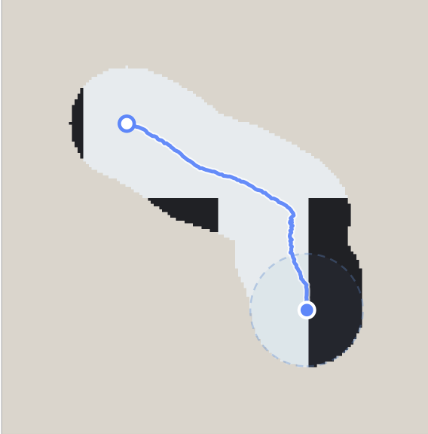
\includegraphics[width=7.0cm,height=2.35cm,keepaspectratio]{phys_try1.png}}; &
  \node[box] (eng0)  {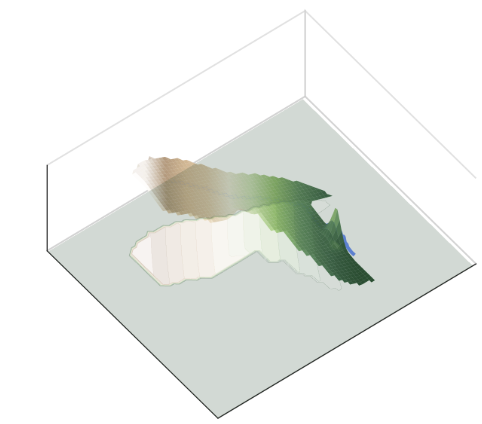
\includegraphics[width=7.0cm,height=2.35cm,keepaspectratio]{energy_try1.png}}; \\

  \node[box] (phys1) {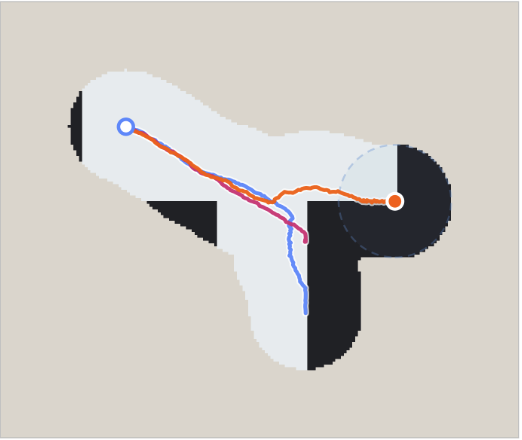
\includegraphics[width=7.0cm,height=2.35cm,keepaspectratio]{phys_try2.png}}; &
  \node[box] (eng1)  {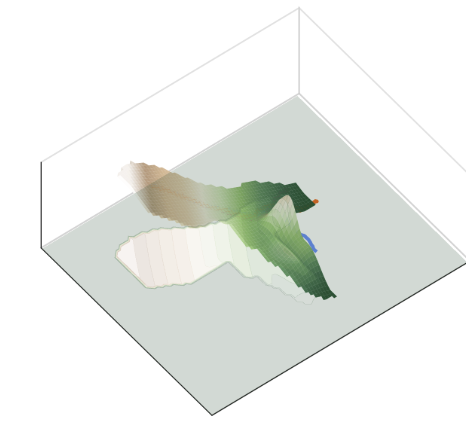
\includegraphics[width=7.0cm,height=2.35cm,keepaspectratio]{energy_try2.png}}; \\

  \node[box] (phys2) {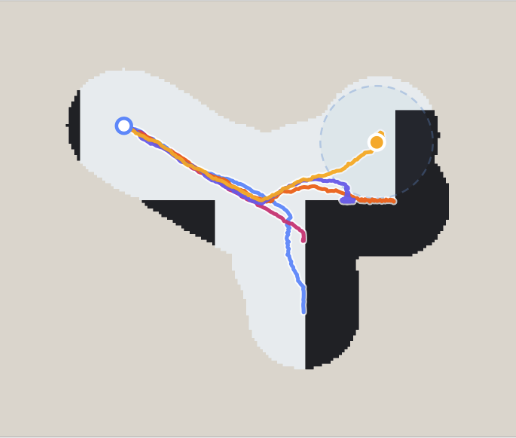
\includegraphics[width=7.0cm,height=2.35cm,keepaspectratio]{phys_try3.png}}; &
  \node[box] (eng2)  {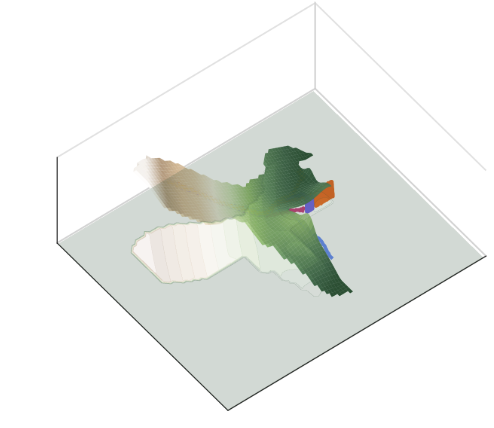
\includegraphics[width=7.0cm,height=2.35cm,keepaspectratio]{energy_try3.png}}; \\
};

\node[header, text width=4.5cm, anchor=south] (colL) at ($(phys0.north)+(0,7mm)$)
{Physical space\\(unknown $\rightarrow$ revealed by local sensing)};

\node[header, text width=4.0cm, anchor=south] (colR) at ($(eng0.north)+(0,7mm)$)
{Hamiltonian energy terrain\\(learned progressively)};

% ------------------- Title -------------------
\node[font=\small\bfseries, anchor=south]
  at ($(colL.north)!0.5!(colR.north)+(0,2.5mm)$)
{Progressive Hamiltonian Landscape Learning from Local Sensing {along Hamiltonian geodesic pathways}};

% ------------------- Vertical progression arrows -------------------
\draw[arrow] (phys0.south) -- (phys1.north);
\draw[arrow] (phys1.south) -- (phys2.north);
\draw[arrow] (eng0.south) -- (eng1.north);
\draw[arrow] (eng1.south) -- (eng2.north);

% ------------------- Cross-column arrows + boxed labels -------------------
\draw[arrow, accent] (phys0.east) -- (eng0.west)
  node[midway, above=2mm, alabel] {scan local env $\Rightarrow$ build initial $H_{\tau}$};

\draw[arrow, accent2] (phys1.east) -- (eng1.west)
  node[midway, above=2mm, alabel] {Try 1 feedback $\Rightarrow$ update $H_{\tau}$};

\draw[arrow, accent3] (phys2.east) -- (eng2.west)
  node[midway, above=2mm, alabel] {Try 2 feedback $\Rightarrow$ refine $H_{\tau}$};

% ------------------- Bottom idea box -------------------
\node[draw, rounded corners=2pt, thick, fill=black!1,
      inner sep=6pt, text width=13cm, align=center, anchor=north]
  at ($(G.south)+(0,-11mm)$) {
  \textbf{Idea:} In an unknown environment, the agent repeatedly senses a \emph{local} neighborhood,
  attempts to reach the stage goal, and incrementally learns a Hamiltonian energy landscape whose valleys guide future attempts under partial observability.
};

\end{tikzpicture}
\caption{\textbf{Conceptual overview: progressive energy-landscape shaping from local sensing.}
\textit{Left}: the physical workspace is initially unknown and is revealed only through local sensing around the agent, producing a partial view of nearby obstacles and a stage goal.
\textit{Right}: from this partial context, the agent builds an initial internal “energy terrain” and then repeatedly attempts a short plan toward the stage goal; each attempt produces simple feedback (e.g., collisions/clearance and progress), which is used to refine the terrain. Over successive refinements, the terrain becomes smoother and its low-energy valleys align with traversable corridors, guiding future attempts even under partial observability.}

\label{fig:teaser_progressive_landscape}
\end{figure}



\paragraph{Overview.} 
We address how GRL--SNAM converts an online mapless navigation task into a stagewise {\emph{energy landscape exploration and mapping}} process under dynamical and geometric constraints. The SNAM task is to move a (deformable) robot in 2d space from $\vec x_0\in\mathbb R^2$ to a goal $\vec x_g\in\mathbb R^2$ in an unknown workspace whose obstacles are encoded by an (unknown) occupancy field $I:\mathbb R^2\to\{0,1\}$. The robot is bound with state $\vec q=(\vec y, \vec c, \vec\psi)\in \mathcal{Q}$ where $\vec c\in\mathbb R^2$ parameterize the robot pose in world coordinate, and $\vec y\in \mathbb{R}^{\text{sensor}},\vec\psi\in \mathbb{R}^{\text{robot}}$ collect sensory and deformation/object configuration variables. The configuration space $\mathcal{Q}$ is assumed to be decomposable into three individual configuration space $\mathcal{Q}=\mathcal{Q}_y\times \mathcal{Q}_f\times \mathcal{Q}_o$, with $\vec{y}\in\mathcal{Q}_y$, $\vec{c}\in \mathcal{Q}_f$ and $\vec\psi\in\mathcal{Q}_o$.

{ We assume the navigation system can query an independent sensor and the sensor would return an environment context $\mathcal{E}$ sensed via current configuration} $\vec{q}$\footnote{How to design the best sensory pipeline is out of this paper's discussion. We assume that sensor can always return the context of environment upon giving {its current} configuration $\vec{q}$.}. The context $\mathcal{E}$ at least include a local target goal $\vec{c}_{target}(\mathcal{E})\in \mathbb{R}^{2}$,  an obstacle cardiality $C(\mathcal{E})\in \mathbb{N}$ and $C(\mathcal{E})$ non-collided constraints $\{d_i(\vec{q};\mathcal{E})\geq 0\}_{i=1}^{C(\mathcal{E})}$. Given current stage's context $\mathcal{E}$, GRL--SNAM learns to ``construct" optimal control problems, whose solution offers an optimally controlled path, by learning to map each environment context $\mathcal E_\tau$ at stage $\tau=0,1,2,\ldots,$ into a \textit{reduced Hamiltonian} via a parametrized network $\eta_{\xi}$:
\[
\eta_{\xi}:\mathcal E_\tau \longmapsto H(\cdot;\mathcal E_\tau)\in \mathscr H,
\quad 
\mathscr H\cong C^{\infty}(T^{*}\mathcal{Q},\mathbb{R}),
\]
where $T^{*}\mathcal{Q}$ refers cotangent bundle of $\mathcal{Q}$. An element of $T^{*}\mathcal{Q}$ is a pair $(\vec{q},p)$ with $\vec{q}\in \mathcal{Q}$ and $p\in T^{*}_{\vec{q}}\mathcal{Q}$, where $p$ is a covector (a linear functional)
acting on tangent vectors $\vec{v}\in T_{\vec{q}}\mathcal{Q}$. The \emph{policy} $\pi$, different from conventional RL definition, is denoted as the time-$\Delta t$ flow map induced by Hamiltonian vector field:
\begin{equation}
\pi(\vec{q}|p):=\ \Phi^{\Delta t}_{H}(\vec{q},p),\quad \text{ where } \Phi^{\Delta t}_{H}(\cdot):T^*\mathcal{Q}\to T^*
\mathcal{Q},
\quad (\vec{q}_{t+\Delta t},p_{t+\Delta t})=\Phi^{\Delta t}_{H}(\vec{q}_{t},p_{t}).
\end{equation}


It then treats a SNAM problem as finding three policies operating at different effective timescales of each subsystem by decomposing $H$ into three Hamiltonians $H_y:T^{*}\mathcal{Q}_y\rightarrow \mathbb{R}$, $H_f:T^{*}\mathcal{Q}_f\rightarrow \mathbb{R}$ and $H_o:T^{*}\mathcal{Q}_o\rightarrow \mathbb{R}$. 
 \begin{enumerate}[i.)]
     \item a {\emph{sensing policy}} $\pi_y: T^*\mathcal{Q}_y\to T^*
\mathcal{Q}_y$ that maintains how to update sensor configuration to acquire environment representation and active collision constraints from partial observations;
     \item a \emph{frame policy} $\pi_f:  T^*\mathcal{Q}_f\to T^*
\mathcal{Q}_f$ that plans short-horizon motion in local frames toward intermediate “stage” goal $\vec{c}_{target}$;
     \item a \emph{shape policy} $\pi_o: T^*\mathcal{Q}_o\to T^*\mathcal{Q}_o$ that modulates the robot’s morphology (e.g., deformation or scale) to exploit narrow passages.
 \end{enumerate}
 Rather than stacking these as a manually tuned hierarchy, we treat each policy as a flow map with its own energy terms under a shared latent codex of sensored environments. We denote $g_{\xi}$, which contains both $\eta_{\xi}$ and policy specific parameter (discussed in \cref{subsec:modular_architecture}), as the overall navigator function of GRL--SNAM. GRL--SNAM further separates learning $g_{\xi}$ into complementary regimes: \emph{offline}, we train reference Hamiltonians on trajectory data to capture fundamental couplings between sensing, planning, and deformation in local frames;
\emph{online}, we adapt open-loop control terms that reweight fixed energy components and add minimal non-conservative corrections injected into policies. Formally, offline learning yields a initial reference reduced Hamiltonian $H$ per local scenario $\mathcal{E}$, and online adaptation performs geometric alignment by updating $\pi_k,k\in\{s,f,o\}$. This realizes a conservative adaptation principle: systems default to learned physics-based behavior while adding just enough correction to handle new obstacles or map updates, rather than catastrophically relearning policies. \cref{algo:online_grl_snam_main:short} shows the overall pipeline. \cref{alg:meta_training} discuss how to obtain $g_{\xi}$ offline. The full pseudo-code, including initialization, query protocols, energy assembly, integration details, and adaptation rules, is deferred to Algorithm~\ref{algo:online_grl_snam} in Appendix~\ref{app:algorithm_details}.


\begin{algorithm}[h!]
\caption{Online GRL-SNAM pipeline}
\label{algo:online_grl_snam_main:short}
\begin{algorithmic}[1]
\State \textbf{Input:} goal $\mathbf{x}_g$, initial $z_0=(q_0,p_0)$ (typically $p_0{=}0$), step $\tau$, horizons $(T_y,T_f,T_o)$, max steps $N_{\max}$
\State \textbf{Init:} $n\!\leftarrow\!0$, environment $\mathcal{E}_0$, environment counter $\tau\gets 0$ active set $\mathcal{C}_0\!\leftarrow\!\emptyset$
\State \textbf{Init:} meta state $(\eta_0,\mu_0,u_{f,0})$ from network $g_\xi$,
\State Assemble $H$ by computing $g_{\xi}(\mathcal{E}_{0})$
\While{$\neg$\textsc{ReachedGoal}$(\vec{c}_n,\mathbf{x}_g)$ \textbf{and} $n<N_{\max}$}
    
    \If{$n \equiv 0 \pmod{T_y}$}   
        \State Assemble $H_y$, provide $z_{y,0}$.
        \State Query Sensor Process via $\pi_y$ and get response $\mathsf{R}_y$
    \EndIf
    \If{$n \equiv 0 \pmod{T_f}$}
        \State Assemble $H_f$, $u_{f}^{\xi,n}, \mu_{f}^{\xi,n}$, provide $z_{f,0}$.
        \State Query Free Path Extractor via $\pi_f$ and get response $\mathsf{R}_f$
    \EndIf
    \If{$n \equiv 0 \pmod{T_o}$}
        \State Assemble $H_o$, provide $z_{o,0}$.
        \State Query Shape Reconfig via $\pi_o$ and get response $\mathsf{R}_o$
    \EndIf
    \State Collect QoIs $y_n$ from responses $\mathsf{R}_y$, $\mathsf{R}_f$ and $\mathsf{R}_o$.
    \State Compute correction term $u_f^{\xi,n}$ via $y_n$.
    \If{$n \equiv 0 \pmod{T_y}$ \textbf{or} reach stage goal}
    \State Update $\mathcal{E}_{\tau+1}$ via response $\mathsf{R}_y$.
    \State Reassemble $H$ by computing $g_{\xi}(\mathcal{E}_{\tau+1})$
    \State $\tau\gets \tau+1$
    \EndIf
    \State $n\leftarrow n+1$
\EndWhile
\State \textbf{Return:} trajectory $\{z_n\}_{n=0}^{N}$ and parameter history $\{(\eta_n,\mu_{f}^{\xi,n},u_{f}^{\xi,n})\}_{n=0}^{N}$
\end{algorithmic}
\end{algorithm}


\subsection{Navigation as Hamiltonian Optimization}
\label{subsec:problem_formulation}
\paragraph{From a stagewise constrained optimal control problem to a reduced Hamiltonian system.}
At a fixed stage $\tau$ and local scenario $\mathcal E_\tau$, we model motion planning for the deformable robot state
$\vec q\in Q$ as a \emph{constrained optimal control problem}:
\begin{equation}
\label{eq:motion:planning:continuous:original:form}
\min_{\vec u(\cdot)\in\mathcal U}\ \int_0^{T} L(\vec q(t),\vec u(t),t;\mathcal E_\tau)\,dt
\quad
\text{s.t.}\;
\begin{cases}
\dot{\vec q}(t)= v(\vec q(t),\vec u(t),t;\mathcal E_\tau), \\
d_i(\vec q(t);\mathcal E_\tau)\ge 0,\quad i=1,2,\ldots, C(\mathcal E_\tau), \\
\vec q(0)=\vec q_0,\quad \vec q(T)=\vec q_{\text{target}}(\mathcal E_\tau).
\end{cases}
\end{equation}
Here $\vec q_0$ is inherited from the previous stage $\mathcal E_{\tau-1}$ (or initialized as $(\vec x_0,\vec 0,\vec 0,\vec 0)$ for $\tau=1$),
and $\vec q_{\text{target}}(\mathcal E_\tau)$ is a local goal specified by the stagewise planner.
The inequality constraints $d_i(\vec q;\mathcal E_\tau)\ge 0$ encode collision avoidance with the locally sensed geometry;
their number $C(\mathcal E_\tau)$ and active subset may vary across scenarios.
Under standard regularity assumptions, a necessary condition for optimality in \cref{eq:motion:planning:continuous:original:form}
is given by the \emph{state-constrained Pontryagin maximum principle(PMP)} \citep{FERREIRA1994whenpmp, hartl1995survey, pearson1966discrete}.
We summarize the resulting reduction to a Hamiltonian system below (a formal statement and proof are provided in
\cref{thm:forward_state_constrained_pmp_reduced_ham}).

\begin{lemma}
\label{thm:fwd_pmp_to_reduced_ham:short}
Consider \cref{eq:motion:planning:continuous:original:form} and assume:
(i) control-affine dynamics $v(\vec q,\vec u,t;\mathcal E)=f(\vec q;\mathcal E)+A(\vec q;\mathcal E)\,u$,
(ii) separable running cost $L(\vec q,\vec u,t;\mathcal E)=\ell(\vec q;\mathcal E)+\varphi(\vec u)$ with $\varphi$ proper, closed, and strictly convex,
and (iii) the regularity/qualification conditions required for the state-constrained maximum principle.
Then there exist a costate $p:[0,T]\to\mathbb R^{\dim Q}$ of bounded variation and nonnegative Radon measures
$\{\mu_i\}_{i=1}^{C(\mathcal E_\tau)}$ such that, defining the reduced Hamiltonian
\begin{equation}
\label{eq:reduced_ham_short}
H_{PMP}(\vec{q},p;\mathcal E):=\ell(\vec{q};\mathcal E)+p^\top f(\vec{q};\mathcal E)+\varphi^\ast\!\big(A(\vec{q};\mathcal E)^\top p\big),
\end{equation}
the optimality conditions can be written (in measure form) as
\begin{equation}
\label{eq:reduced_ham_flow_short}
\begin{aligned}
\dot{\vec{q}}^{\star}(t)&=\nabla_p H_{PMP}\big(\vec{q}^{\star}(t),p(t);\mathcal E\big),\\
dp(t)&= -\nabla_q H_{PMP}\big(\vec{q}^{\star}(t),p(t);\mathcal E\big)\,dt
-\sum_{i=1}^{C(\mathcal E)} \nabla d_i\!\big(\vec{q}^\star(t);\mathcal E\big)\,\mu_i(dt).    
\end{aligned}
\end{equation}
In particular, on interior intervals where all constraints are inactive, $\mu_i\equiv 0$ and \cref{eq:reduced_ham_flow_short}
reduces to the classical Hamiltonian system $\dot{\vec{q}}^\star=\nabla_p H$, $\dot p=-\nabla_{\vec{q}} H$.
\end{lemma}

\paragraph{Barrier relaxation and the learnable {sub-modular} Hamiltonian.}
For learning and differentiable rollout, we employ a smooth barrier relaxation of the state constraints \citep{NocedalWright2006NumericalOptimization}.
Let $b_i:\mathbb R\to\mathbb R$ be a $C^2$ barrier potential applied to the clearance $d_i(q;\mathcal E)$, and let
$\alpha_i(\mathcal E)\ge 0$ be environment-conditioned weights.
Define the \emph{barrier-shaped} running cost
\begin{equation}
\label{eq:barrier_shaped_cost}
L_{\alpha}(q,u;\mathcal E)
:=\ell(q;\mathcal E)+\varphi(u)+\sum_{i=1}^{C(\mathcal E)} \alpha_i(\mathcal E)\, b_i\!\big(d_i(q;\mathcal E)\big),
\end{equation}
which yields an \emph{unconstrained} OCP that approximates \cref{eq:motion:planning:continuous:original:form} as the barriers stiffen.
Applying the reduction in \cref{cor:mechanical_reduced_hamiltonian} (quadratic $\varphi$ and $f\equiv 0$)
leads to the PMP Hamiltonian
\begin{equation}
\label{eq:def:pmp:hamiltonian:grl-snam}
H_{PMP}(q,p;\mathcal E)
=\tfrac12\,p^\top M^{-1}p- V(q;\mathcal E),
\quad
V(q;\mathcal E)
:= \ell(q;\mathcal E)+\sum_{i=1}^{C(\mathcal E)} \alpha_i(\mathcal E)\, b_i\!\big(d_i(q;\mathcal E)\big),
\end{equation}
where $M\in\mathbb S_{++}^2$ is the (learned or fixed) mass/metric induced by the control penalty. We commented on \cref{prop:barrier_convergence} that under certain assumptions log-barrier relaxed OCPs can recover the constrained OCP. The statement of the proposition is inspired from \citet{malisani2023interior}.

\begin{proposition}[Barrier relaxation converges to the state-constrained OCP (log-barrier)]
\label{prop:barrier_convergence}
Fix a scenario $\mathcal E$ and consider the state-constrained OCP
\begin{equation}
\begin{aligned}
\min_{u(\cdot)}&\ J(u):=\int_0^T L(q(t),u(t),t;\mathcal E)\,dt
\\ \text{s.t.}&\quad
\dot q=f(q;\mathcal E)+A(q;\mathcal E)u,\ \ d_i(q(t);\mathcal E)\ge 0\ \forall t,\ \ q(0)=q_0,\ q(T)=q_T.    
\end{aligned}
\end{equation}

Assume:
(A1) (\emph{Slater}) there exists a strictly feasible trajectory, i.e., some admissible $(\bar q,\bar u)$ with
$d_i(\bar q(t);\mathcal E)\ge \delta$ for all $t\in[0,T]$ and all $i$, for some $\delta>0$;
(A2) $f,A,L,d_i$ are $C^2$ in $q$ (and $L$ is convex in $u$), and the constrained OCP admits a (locally) optimal solution
$(q^\star,u^\star)$ satisfying a suitable constraint qualification and second-order sufficient conditions.

For $t>0$, define the \emph{log-barrier relaxed} (unconstrained) OCP
\[
\min_{u(\cdot)}\ J_t(u):=\int_0^T \Big(
L(q(t),u(t),t;\mathcal E)\;+\;\frac{1}{t}\sum_{i=1}^{C(\mathcal E)} \alpha_i(\mathcal E)\, \phi(d_i(q(t);\mathcal E))
\Big)\,dt,
\quad
\phi(s):=-\log s,
\]
subject only to the dynamics and boundary conditions (and implicitly $d_i(q(t);\mathcal E)>0$ due to $\phi$).
Let $(q^t,u^t)$ be a (locally) optimal solution of the barrier subproblem.

Then:
\begin{enumerate}
\item (\emph{Strict feasibility}) For each $t$, $d_i(q^t(t);\mathcal E)>0$ for all $t\in[0,T]$ and all $i$.
\item (\emph{Convergence of primal variables}) Any sequence $t_k\to\infty$ has a subsequence (not relabeled) such that
$(q^{t_k},u^{t_k})$ converges (in a topology appropriate for the OCP, e.g.\ $q^{t_k}\to q^\star$ strongly and $u^{t_k}\rightharpoonup u^\star$ weakly)
to a (locally) optimal solution $(q^\star,u^\star)$ of the original state-constrained OCP.
\item (\emph{Recovery of multipliers}) Define the barrier-induced (approximate) multipliers
\[
\lambda_i^t(\tau)\ :=\ \frac{\alpha_i(\mathcal E)}{t}\,\frac{1}{d_i(q^t(\tau);\mathcal E)}\ \ge 0.
\]
Along the same subsequence, $\lambda_i^{t_k}$ converges (weakly$^\ast$) to a nonnegative multiplier $\lambda_i^\star$
appearing in the state-constrained PMP/KKT system of the original OCP; moreover complementarity holds in the limit:
$\lambda_i^\star(\tau)\,d_i(q^\star(\tau);\mathcal E)=0$ for a.e.\ $\tau$.
\end{enumerate}
\end{proposition}

\begin{proof}
Defer to \cref{prop:barrier_to_state_constrained_complete}.
\end{proof}

\paragraph{Our geometric reinforcement learning framework.}

GRL-SNAM {learns} a scenario-to-energy map $\mathcal E\mapsto H(\cdot;\mathcal E)$. With a costate initialized, the resulting phase-space integrator
$x_{t+1}=\Phi_{\eta}^{\Delta t}(x_t;\mathcal E)$ with $x_t=(q_t,p_t)$ produces a feasible start-to-goal rollout using only forward passes. We view our proposed method as an Energy-Based Model \citep{hopfield1982neural,ackley1985learning,lecun2006tutorial} yet with augmented search space considering geometric structure of energy landscape \citep{nguyen2025stochastic, ryan2025bayesian, mclennan2025learning}. For deterministic dynamics $\dot q=f(q)+A(q)u$ and cost minimization, the value function satisfies the HJB equation
\[
-\partial_t \mathcal V^{*}(t,q;\mathcal E)
=\inf_{u\in U}\Big\{L(q,u;\mathcal E)+\nabla_q\mathcal V^{*}(t,q;\mathcal E)^\top\big(f(q)+A(q)u\big)\Big\},
\qquad
\mathcal V^{*}(T,q;\mathcal E)=\delta_{q_T}(q).
\]
When $\mathcal V^{*}$ is smooth, the PMP costate admits the feedback representation
$p(t)=\nabla_q\mathcal V^{*}(t,q(t);\mathcal E)$ but one needs to solve the space-time PDE backward in time.
Conventional RL methods approximate $\mathcal V^{*}$ via Bellman recursion/backups, and explore its stochastic counterpart. Our design principle is that the optimal motion could be generated by a forward dynamics. To this end, we propose to learn a generalized Hamiltonian dynamical system whose reduced Hamiltonian is defined as:
\begin{equation}
\label{eq:def:reduced:hamiltonian:grl-snam}
H(q,p;\mathcal E)
=\tfrac12\,p^\top M^{-1}p + \mathcal{R}(q;\mathcal E),
\quad
\mathcal{R}(q;\mathcal E)
:= \ell(q;\mathcal E)+\sum_{i=1}^{C(\mathcal E)} \alpha_i(\mathcal E)\, b_i\!\big(d_i(q;\mathcal E)\big).
\end{equation}
The sign of potential term is reversed as we are approximating the feedforward dynamics using $\nabla_q H$, and the flow reversibility is addressed in \cref{lem:mech_time_reversal}. It lies in the least action principle energy space we want to search, and we address the search space immediately below. 


\paragraph{Search space for the Hamiltonian.}

    The Hamiltonian defined in \cref{eq:def:reduced:hamiltonian:grl-snam} is a function on the cotangent bundle $T^{*}Q$:
\[
H \in \mathscr{H}:=\big\{\,H(q,p;\mathcal{E})=\tfrac12\,p^\top M^{-1}p\;+\;\mathcal{R}(q;\mathcal{E}) 
\ \big|\ M\in \mathbb{S}_{++}^2,\ \mathcal{R}\in \mathscr{R} \,\big\}.
\]
We regard $\mathscr{R}$ as a Hilbert space containing admissible potentials. For 2d navigation we \emph{restrict} the potential space $\mathscr{R}\cong \mathbb{R}^{\vert \xi\vert}$ by defining a parametrized map $\mathcal E\!\to\!\eta_{\xi}(\mathcal E)$ producing
nonnegative dual weights that shape the primal potential. This particular choice is compatible with soft barrier potential addition addressed in \cref{eq:def:reduced:hamiltonian:grl-snam}. In general, each energy
term may itself be parametrized:
\[
H(q,p;\omega,\xi,\mathcal E)\;=\;\tfrac12\,p^\top M(\omega_M)^{-1}p
\;+\;\mathcal{R}(q;\omega,\eta_{\xi}(\mathcal E)),
\]
\vspace{-0.75ex}
\begin{equation}
\begin{aligned}
\mathcal{R}(q;\omega, \eta_{\xi}(\mathcal E))\;&=\;
E_{\mathrm{sensor}}(q;\mathcal{E},\omega_y)+ 
\beta(\mathcal E)\,E_{\mathrm{goal}}(q;\mathcal E,\omega_g)
+\lambda(\mathcal E)\,E_{\mathrm{obj}}(q;\omega_d)
\\
&+\sum_{i\in\mathcal C(\mathcal E,q)} \alpha_i(\mathcal E)\,
b\big(d_i(q;\mathcal E);\omega_b\big),
\end{aligned}
\end{equation}
with $\eta_{\xi}(\mathcal E)\!=\!(\beta(\mathcal E),\lambda(\mathcal E),\{\alpha_i(\mathcal E)\})\in\mathbb R_+^{\,m(\mathcal E)}$.
Here $\omega\!=\!(\omega_y,\omega_M,\omega_g,\omega_d,\omega_b)$ are \emph{intra-term} parameters
(e.g.\ metric, goal shape, deformation model, barrier template), while $\eta_\xi$
learns the \emph{inter-term} tradeoffs by mapping the environment $\mathcal E$
to dual weights. The cardinality $m(\mathcal E)=2+|\mathcal C(\mathcal E,q)|$ is
environment/active-set dependent, so $\eta_\xi$ is implemented with a permutation-invariant
set encoder that outputs per-constraint scores
$\alpha_i(\mathcal E,t)\!\ge\!0$, together
with scalars $\beta(\mathcal E),\lambda(\mathcal E)\!\ge\!0$. The active set $\mathcal{C}(\mathcal{E},q):=\{i~|~d_i(q,\mathcal{E})\leq \hat{d}\}$ is discovered online by sensing. We explain role of each potential term in \cref{fig:energy_decomposition}.


\begin{figure}[htbp]
\centering
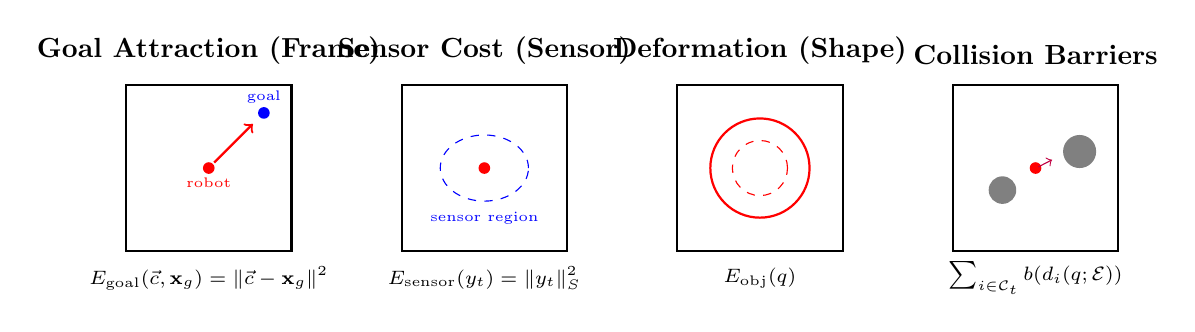
\begin{tikzpicture}[scale=0.7]

% Goal Attraction (Frame Policy)
\begin{scope}[shift={(-7.5,2)}]
    \draw[thick] (-1.5,-1.5) rectangle (1.5,1.5);
    \node[above] at (0,1.7) {\textbf{Goal Attraction (Frame)}};
    \fill[red] (0,0) circle (3pt) node[below] {\tiny robot};
    \fill[blue] (1,1) circle (3pt) node[above] {\tiny goal};
    \draw[->,thick,red] (0.1,0.1) -- (0.8,0.8);
    \node at (0,-2) {\scriptsize $E_{\mathrm{goal}}(\vec{c},\mathbf{x}_g) = \|\vec{c}-\mathbf{x}_g\|^2$};
\end{scope}

% Sensor Cost (Sensor Policy)
\begin{scope}[shift={(-2.5,2)}]
    \draw[thick] (-1.5,-1.5) rectangle (1.5,1.5);
    \node[above] at (0,1.7) {\textbf{Sensor Cost (Sensor)}};
    \fill[red] (0,0) circle (3pt);
    \draw[blue,dashed] (0,0) ellipse (0.8 and 0.6);
    \node[blue] at (0,-0.9) {\tiny sensor region};
    \node at (0,-2) {\scriptsize $E_{\mathrm{sensor}}(y_t)=\|y_t\|_{S}^2$};
\end{scope}

% Deformation (Shape Policy)
\begin{scope}[shift={(2.5,2)}]
    \draw[thick] (-1.5,-1.5) rectangle (1.5,1.5);
    \node[above] at (0,1.7) {\textbf{Deformation (Shape)}};
    \draw[red,thick] (0,0) circle (0.9);   % expanded radius
    \draw[red,dashed] (0,0) circle (0.5); % contracted radius
    \node at (0,-2) {\scriptsize $E_{\mathrm{obj}}(q)$};
\end{scope}

% Collision Barriers
\begin{scope}[shift={(7.5,2)}]
    \draw[thick] (-1.5,-1.5) rectangle (1.5,1.5);
    \node[above] at (0,1.7) {\textbf{Collision Barriers}};
    \fill[red] (0,0) circle (3pt);
    \fill[gray] (0.8,0.3) circle (0.3);
    \fill[gray] (-0.6,-0.4) circle (0.25);
    \draw[->,purple] (0.05,0.02) -- (0.3,0.15);
    \node at (0,-2) {\scriptsize $\sum_{i\in\mathcal{C}_t} b(d_i(q;\mathcal{E}))$};
\end{scope}

\end{tikzpicture}
\caption{
Policy-aligned energy decomposition in GRL--SNAM.
The sensor policy exposes a sensor configuration cost $E_{\mathrm{sensor}}$, 
the frame policy induces goal attraction $E_{\mathrm{goal}}$, 
and the shape policy contributes deformation energy $E_{\mathrm{obj}}$, 
while all modules share collision barrier terms $b(d_i)$ around active constraints $\mathcal{C}_t$.
A meta-policy $g_\xi$ assigns weights $(\beta,\lambda,\{\alpha_i\})$ to these components to form the surrogate potential
$\mathcal{R}(q;\eta_\xi^t,\mathcal{E}) = E_{\mathrm{sensor}} + \beta^t E_{\mathrm{goal}} + \lambda^t E_{\mathrm{obj}} + \sum_{i\in\mathcal{C}_t} \alpha_i^t b(d_i)$
used in the Hamiltonian dynamics.
}
\label{fig:energy_decomposition}
\end{figure}


\subsection{Navigator score fields and context-conditioned policies.}
\label{subsec:modular_architecture}

Rather than learning a single monolithic mapless navigation policy, we decompose each module of robots by a small collection of
\emph{module score fields} defined on phase space. Each module is a context-conditioned Hamiltonian system: its energy
induces a vector field, and the time-$\Delta t$ flow map of that vector field serves as the module's policy operator.

\paragraph{Sub-Modular score fields and induced policies.}
%\label{def:module_score_fields}
Let $\mathcal K=\{y,f,o\}$ index the sensor, frame, and shape modules. For each $k\in\mathcal K$, let $Q_k$ denote its
configuration manifold and let $\mathcal Z_k:=T^*\mathcal{Q}_k$ be its phase space with state $z_k=(q_k,p_k)$, where
$q_k\in \mathcal{Q}_k$ and $p_k\in T^*_{q_k}\mathcal{Q}_k$ is the conjugate costate.
Let $\theta_k\in\Theta_k$ denote the module-specific parameters, and assume the parameter sets are disjoint:
$\Theta_i\cap\Theta_j=\emptyset$ for all $i\neq j$.
Let $\mathcal E\in\mathscr E$ denote a local environment context (e.g., a local observation patch together with a goal descriptor).
We model the module energy by a differentiable Hamiltonian surrogate
\[
 h_k^{\theta_k}:\ \mathcal Z_k\times\mathscr E\times\mathbb R_{\ge 0}\to\mathbb R,\qquad (z_k,\mathcal E,t)\mapsto h_k^{\theta_k}(z_k;\mathcal E,t),
\]
where $t$ denotes the (local) integration time within a short rollout horizon.
Given a context-conditioned damping matrix $\Gamma_k^{\xi}(q_k;\mathcal E)\succeq 0$ and a nonconservative input
$G_k^{\xi}(q_k;\mathcal E)\,u_k^{\xi}(z_k,t;\mathcal E)$, { we define the \emph{modular score field} (deterministic drift) as the differential Hamiltonian 
{\small
\begin{equation}
\label{eq:module_score_field}
 s_k^{\theta_k,\xi}(z_k,t;\mathcal E)
 \!:=\!
 \begin{bmatrix}
 \nabla_{p_k} h_k^{\theta_k}(z_k;\mathcal E,t)\\
 -\nabla_{q_k} h_k^{\theta_k}(z_k;\mathcal E,t)
 \end{bmatrix}
 \!+\!
 \begin{bmatrix}
 0\\
 -\Gamma_k^{\xi}(q_k;\mathcal E)\,\nabla_{p_k} h_k^{\theta_k}(z_k;\mathcal E,t)+G_k^{\xi}(q_k;\mathcal E)\,u_k^{\xi}(z_k,t;\mathcal E)
 \end{bmatrix}.
\end{equation}
}
The modular stagewise} dynamics are the ODE $\dot z_k=s_k^{\theta_k,\xi}(z_k,t;\mathcal E)$.
Fix an integration rule with step size $\Delta t>0$ and denote by $\Phi_{k}^{\Delta t}(\cdot;\mathcal E):\mathcal Z_k\to\mathcal Z_k$
its time-$\Delta t$ flow map.
We define the (deterministic) \emph{context-conditioned modular policy} as the rollout operator
\begin{equation}
\label{eq:module_policy_operator}
 \pi_k^{\theta_k,\xi}(\mathcal E):=\Phi_{k}^{\Delta t}(\cdot;\mathcal E),\qquad z_{k,t+\Delta t}=\pi_k^{\theta_k,\xi}(\mathcal E)(z_{k,t}).
\end{equation}
If $\Gamma_k^{\xi}\equiv 0$ and $u_k^{\xi}\equiv 0$, then $s_k^{\theta_k,\xi}$ reduces to the Hamiltonian vector field and
$\pi_k^{\theta_k,\xi}(\mathcal E)$ is symplectic; otherwise it remains a (local) diffeomorphism under standard Lipschitz
regularity but is generally non-symplectic.

The disjointness of parameter sets implies $\partial s_k^{\theta_k,\xi}/\partial\theta_j\equiv 0$ for all $j\neq k$,
so the intra-modular energies can be trained in parallel while coordination is enforced through shared context-dependent
constraints and shared dual weights.

\paragraph{Template {Sub-modular} Hamiltonians and shared dual weights.}
We couple modules through a shared mechanical energy family and context-conditioned potential { reshaping}.
Let $\eta(\mathcal E)=\eta_{\xi}(\mathcal E)\in\mathbb R_+^{m(\mathcal E,t)}$ denote the nonnegative dual weights produced by
the navigator's context encoder, with components
$\eta(\mathcal E)=(\beta(\mathcal E),\lambda(\mathcal E),\{\alpha_i(\mathcal E,t)\}_{i\in\mathcal C_t})$.
The active constraint set $\mathcal C_t(\mathcal E,q):=\{i\mid d_i(q;\mathcal E)\ge 0\}$ is discovered online by sensing.
For each $k\in\mathcal K$ we use a mechanical template
\begin{equation}
\label{eq:module_template_hamiltonian}
 H_k(q_k,p_k;\mathcal E)
 =\tfrac12\,p_k^\top M^{-1}p_k+\mathcal R_k(q_k;\eta(\mathcal E),\mathcal E), \quad h_k^{\theta_k}(z_k;\mathcal{E},0)=H_k(z_k;\mathcal{E}).
\end{equation}
and instantiate the context-shaped potentials
\begin{align}
\label{eq:module_potentials}
 \mathcal R_y(q_y;\eta,\mathcal E)
 &=E_{\mathrm{sensor}}(q_y;\mathcal E,\omega_y)
 +\sum_{i\in\mathcal C_t(\mathcal E,q_y)}\alpha_i(\mathcal E,t)\,b\!\big(d_i(q;\mathcal E);\omega_b\big),\\
 \mathcal R_f(q_f;\eta,\mathcal E)
 &=\beta(\mathcal E)\,E_{\mathrm{goal}}(q_f;\mathcal E,\omega_g)
 +\sum_{i\in\mathcal C_t(\mathcal E,q_f)}\alpha_i(\mathcal E,t)\,b\!\big(d_i(q;\mathcal E);\omega_b\big),\\
 \mathcal R_o(q_o;\eta,\mathcal E)
 &=\lambda(\mathcal E)\,E_{\mathrm{obj}}(q_o;\omega_d)
 +\sum_{i\in\mathcal C_t(\mathcal E,q_o)}\alpha_i(\mathcal E,t)\,b\!\big(d_i(q;\mathcal E);\omega_b\big).
 \label{eq:module_template_potential:o}
\end{align}
Here $\omega=(\omega_y,\omega_g,\omega_d,\omega_b)$ collects intra-term parameters, while $\eta(\mathcal E)$ controls
inter-term tradeoffs via nonnegative weights.

\paragraph{{Sub-modular} responses and aggregation.}
Each module integrates its phase dynamics over a short horizon and returns a standardized response map $\mathsf R_k$  to the navigator. The navigator aggregates these responses to update $\eta_{\xi}(\mathcal E)$ (and, when enabled,
damping/correction parameters) and to generate stable trajectories across stages.

\begin{figure}[h]
\centering
\resizebox{\linewidth}{!}{%
\begin{tikzpicture}[
  node distance=0.5cm,
  font=\small,
  % --- Colors ---
  sensorcolor/.style={draw=RoyalBlue, fill=RoyalBlue!10},
  framecolor/.style ={draw=Crimson,   fill=Crimson!10},
  shapecolor/.style ={draw=ForestGreen,fill=ForestGreen!10},
  navcolor/.style   ={draw=Orange,    fill=Orange!10},
  band/.style       ={fill=black!3, draw=none},
  % --- Styles ---
  mod/.style   ={rectangle,rounded corners=2pt,draw,very thick,align=center,
                 minimum width=4.8cm,minimum height=2.2cm,#1},
  nav/.style   ={rectangle,rounded corners=2pt,draw,very thick,align=center,
                 minimum width=14.0cm,minimum height=2.0cm,#1},
  io/.style    ={circle,draw,thick,inner sep=0pt,minimum size=2.8mm,fill=white},
  qarr/.style  ={thick,dashed,-{Stealth[length=2.2mm]}},
  rarr/.style  ={thick,-{Stealth[length=2.2mm]}},
  chip/.style  ={rectangle,rounded corners=1pt,draw,thin,inner sep=2pt,
                 font=\scriptsize,fill=white},
  dsicon/.style={rectangle,draw,thin,fill=white,minimum width=4.5mm,minimum height=4.5mm},
  badge/.style ={circle,draw,thin,fill=white,minimum size=5mm,font=\scriptsize\bfseries},
  xtiny/.style ={font=\scriptsize},
  response/.style={rectangle,draw,thin,fill=white,rounded corners=1pt,font=\scriptsize,align=left,inner sep=3pt}
]

% ====== GRID COORDS ======
\coordinate (ColY) at (-5.2,0);   % Sensor column x
\coordinate (ColF) at ( 0.0,0);   % Frame column x
\coordinate (ColO) at ( 5.2,0);   % Shape column x

% ====== Background band ======
\node[rectangle,band,minimum width=16.5cm,minimum height=2.8cm,anchor=center] at (0,6.0) {};

% ====== MODULES (moved up) ======
% Sensor module
\node[mod=sensorcolor,anchor=center] (sensor) at ($(ColY)+(0,6.0)$) {
    {\bfseries\color{RoyalBlue}Sensor Policy $\pi_y^{\theta_y,\xi}$}\\[2pt]
    {\scriptsize $s_y^{\theta_y,\xi}(z_y,t;\mathcal{E})=\mathbb{J}\nabla_{z_y}h_y^{\theta_y}$}\\[1pt]
    {\scriptsize\color{gray} $\Gamma_y^\xi\equiv 0,\; G_y^\xi u_y^\xi\equiv 0$}
};

% Frame module
\node[mod=framecolor,anchor=center] (frame) at ($(ColF)+(0,6.0)$) {
    {\bfseries\color{Crimson}Frame Policy $\pi_f^{\theta_f,\xi}$}\\[1pt]
    {\scriptsize $s_f^{\theta_f,\xi}=\mathbb{J}\nabla_{z_f}h_f^{\theta_f}+\begin{bmatrix}0\\-\Gamma_f^\xi\dot{q}_f+G_f^\xi u_f^\xi\end{bmatrix}$}\\[1pt]
    {\scriptsize\color{gray} $\Gamma_f^\xi=\mu_\xi(\mathcal{E})\mathbf{I},\; G_f^\xi=\mathbf{I}$}
};

% Shape module
\node[mod=shapecolor,anchor=center] (shape) at ($(ColO)+(0,6.0)$) {
    {\bfseries\color{ForestGreen}Shape Policy $\pi_o^{\theta_o,\xi}$}\\[2pt]
    {\scriptsize $s_o^{\theta_o,\xi}(z_o,t;\mathcal{E})=\mathbb{J}\nabla_{z_o}h_o^{\theta_o}$}\\[1pt]
    {\scriptsize\color{gray} $\Gamma_o^\xi\equiv 0,\; G_o^\xi u_o^\xi\equiv 0$}
};

% ====== Configuration space icons (top-left inside each) ======
\foreach \M/\L in {sensor/$\mathcal{Q}_y$,frame/$\mathcal{Q}_f$,shape/$\mathcal{Q}_o$}{
  \node[dsicon] (ds-\M) at ([xshift=4mm,yshift=-3mm]\M.north west) {};
  \draw[thin] (ds-\M.south west)++(0,0.6mm) rectangle ++(4.5mm,0.8mm);
  \draw[thin] (ds-\M.south west)++(0,1.8mm) rectangle ++(4.5mm,0.8mm);
  \draw[thin] (ds-\M.south west)++(0,3.0mm) rectangle ++(4.5mm,0.8mm);
  \node[xtiny] at ([xshift=7mm]ds-\M.east) {\L};
}

% ====== Time badges (outside top-right) ======
\node[badge,text=RoyalBlue]   at ([xshift=-14pt,yshift=8pt]sensor.north east) {$T_y$};
\node[badge,text=Crimson]     at ([xshift=-14pt,yshift=8pt]frame.north east)  {$T_f$};
\node[badge,text=ForestGreen] at ([xshift=-14pt,yshift=8pt]shape.north east)  {$T_o$};

% ====== Timescale annotation ======
\node[xtiny,anchor=west] at (8.0,7.6) {$T_y \gg T_f \gg T_o$};

% ====== POTENTIAL TERMS (above modules) ======
\node[chip,fill=RoyalBlue!5] at ([yshift=6pt]sensor.north) {$\mathcal{R}_y: E_{\mathrm{sensor}} + \sum_i\alpha_i b(d_i)$};
\node[chip,fill=Crimson!5] at ([yshift=6pt]frame.north) {$\mathcal{R}_f: \beta E_{\mathrm{goal}} + \sum_i\alpha_i b(d_i)$};
\node[chip,fill=ForestGreen!5] at ([yshift=6pt]shape.north) {$\mathcal{R}_o: \lambda E_{\mathrm{obj}} + \sum_i\alpha_i b(d_i)$};

% ====== RESPONSE BOXES (between modules and navigator) ======
\node[response,fill=RoyalBlue!5] (Ry) at ($(ColY)+(0,3.6)$) {
    $\mathsf{R}_y=\big\{z_{0:T_y}^{(y)},\mathrm{QoI}_y\big\}$\\
    $\mathrm{QoI}_y=\Delta\mathcal{E}$
};
\node[response,fill=Crimson!5] (Rf) at ($(ColF)+(0,3.6)$) {
    $\mathsf{R}_f=\big\{z_{0:T_f}^{(f)},\mathrm{QoI}_f\big\}$\\
    $\mathrm{QoI}_f=\{v_t^{(f)}\}_{t=0}^{T_f}$
};
\node[response,fill=ForestGreen!5] (Ro) at ($(ColO)+(0,3.6)$) {
    $\mathsf{R}_o=\big\{z_{0:T_o}^{(o)},\mathrm{QoI}_o\big\}$\\
    $\mathrm{QoI}_o=\{\min_i d_i\}_{t=0}^{T_o}$
};

% ====== NAVIGATOR ======
\node[nav=navcolor,anchor=center] (nav) at ($(0,1.2)$) {
  {\bfseries Navigator $g_{\xi}$ (Meta-Hamiltonian Composer)}\\[2pt]
  {\scriptsize Tokenize: $\mathcal{T}_t=\mathrm{Tokenize}(\mathcal{C}_t(\mathcal{E},q_t),\,q_t,\,\mathbf{x}_g)$\quad\quad Output: $g_\xi(\mathcal{E})=\big[\,\eta_\xi,\;\mu_\xi,\;u_f^\xi\,\big]$}\\[1pt]
  {\scriptsize Dual weights: $\eta_\xi(\mathcal{E})=(\beta,\lambda,\{\alpha_i\}_{i\in\mathcal{C}_t})$\quad\quad Surrogate: $H=\tfrac{1}{2}p^{\top}M^{-1}p+\mathcal{R}(q;\eta_\xi,\mathcal{E})$}
};

% ====== QUERY ARROWS (Navigator to Modules) ======
\draw[qarr,draw=RoyalBlue]
  ([xshift=-8pt]nav.north-|ColY) -- node[xtiny,fill=white,inner sep=1pt,pos=0.5,left]
  {$(H_y,z_y^t,T_y)$} ([xshift=-8pt]Ry.south-|ColY);

\draw[qarr,draw=Crimson]
  ([xshift=-8pt]nav.north-|ColF) -- node[xtiny,fill=white,inner sep=1pt,pos=0.5,left]
  {$(H_f,z_f^t,T_f,\Gamma_f^\xi,u_f^\xi)$} ([xshift=-8pt]Rf.south-|ColF);

\draw[qarr,draw=ForestGreen]
  ([xshift=-8pt]nav.north-|ColO) -- node[xtiny,fill=white,inner sep=1pt,pos=0.5,left]
  {$(H_o,z_o^t,T_o)$} ([xshift=-8pt]Ro.south-|ColO);

% ====== RESPONSE ARROWS (Response boxes to Navigator) ======
\draw[rarr,draw=RoyalBlue]
  ([xshift=8pt]Ry.south-|ColY) -- ([xshift=8pt]nav.north-|ColY);

\draw[rarr,draw=Crimson]
  ([xshift=8pt]Rf.south-|ColF) -- ([xshift=8pt]nav.north-|ColF);

\draw[rarr,draw=ForestGreen]
  ([xshift=8pt]Ro.south-|ColO) -- ([xshift=8pt]nav.north-|ColO);

% ====== ARROWS from Modules to Response boxes ======
\draw[rarr,draw=RoyalBlue] (sensor.south) -- (Ry.north);
\draw[rarr,draw=Crimson] (frame.south) -- (Rf.north);
\draw[rarr,draw=ForestGreen] (shape.south) -- (Ro.north);

% ====== Environment & Trajectory ======
\node[rectangle,draw,thick,fill=white,minimum width=2.6cm,minimum height=1.0cm,align=center]
      (env) at (-9.2,1.2) {{\bfseries Environment $\mathcal{E}$}\\ {\scriptsize $z_0,\;\mathbf{x}_g,\;\{d_i\geq 0\}$}};
\node[rectangle,draw,thick,fill=white,minimum width=2.6cm,minimum height=1.0cm,align=center]
      (traj) at ( 9.2,1.2) {{\bfseries Trajectory}\\ {\scriptsize $\{z_t\}_{t=0}^{T}$}};

\draw[thick,-{Stealth[length=2.5mm]}] (env.east) -- (nav.west);
\draw[thick,-{Stealth[length=2.5mm]}] (nav.east) -- (traj.west);

% ====== Side annotations ======
% Symplectic matrix definition (left)
\node[rectangle,draw,thin,fill=white,align=left,font=\scriptsize,inner sep=4pt]
      at (-9.8,5.8) {
       \textbf{Symplectic form:}\\[1pt]
       $\mathbb{J}=\begin{bmatrix}0 & I\\-I & 0\end{bmatrix}$\\[1pt]
       $\mathbb{J}\nabla_z h = \begin{bmatrix}\nabla_p h\\-\nabla_q h\end{bmatrix}$
      };

% Online adaptation (right)
\node[rectangle,draw,thin,fill=white,align=left,font=\scriptsize,inner sep=4pt]
      at (10.5,5.8) {
       \textbf{Online observables:}\\[1pt]
       $y_t=[-\mathrm{clr}_t,\mathrm{dist}_t,-\mathrm{speed}_t]^\top$\\[1pt]
       Adapt $\zeta_t=[\eta_t,\mu_t]$ via $J_t\approx\partial y/\partial\zeta$
      };

% ====== Compact Legend ======
\node[rectangle,draw,thick,fill=white,align=left,font=\scriptsize,inner sep=4pt]
      at (0,-0.8) {
       \textbf{Legend:}\;
       \tikz[baseline=-0.5ex]{\node[io]{};} port\quad
       \tikz[baseline=-0.5ex]{\draw[qarr] (0,0)--(8mm,0);} query\quad
       \tikz[baseline=-0.5ex]{\draw[rarr] (0,0)--(8mm,0);} response
       \qquad
       \textbf{Policy as flow:}\; $\pi_k^{\theta_k,\xi}(\mathcal{E}):=\Phi_k^{\Delta t}(\cdot;\mathcal{E})$
      };

\end{tikzpicture}}
\caption{%
Modular score-field architecture for GRL-SNAM.
The Navigator $g_\xi$ tokenizes active constraints $\mathcal{C}_t$, state $q_t$, and goal $\mathbf{x}_g$, then outputs dual weights $\eta_\xi=(\beta,\lambda,\{\alpha_i\})$, friction $\mu_\xi$, and port correction $u_f^\xi$.
Each module $k\in\{y,f,o\}$ integrates its score field $s_k^{\theta_k,\xi}=\mathbb{J}\nabla_{z_k}h_k^{\theta_k}$ (plus non-conservative terms for the frame module) over horizon $T_k$ and returns response $\mathsf{R}_k$ with phase-space rollouts and QoIs.
The frame module uniquely receives dissipation $\Gamma_f^\xi$ and port input $u_f^\xi$; sensor and shape modules have purely symplectic dynamics.
}
\label{fig:independent-score-architecture}
\end{figure}


\subsection{GRL-SNAM offline training and online adaptation}
\label{subsec:navigator_meta_learner}

The GRL-SNAM operates as a meta-learning system that coordinates multi-scale policies by learning how to update their Hamiltonian energy functions rather than directly manipulating phase space states.


\paragraph{Choice of Hamiltonian and Hamiltonian dynamics}
Throughout the paper we further simplify our navigator's Hamiltonian surrogate by assuming fixed $\omega$ throughout all environment when we primarily focus on learning to optimize the
environment-indexed linear cone generated by task energies. The potential energy is denoted as follows and is shown in Figure \ref{fig:energy_decomposition}:  
\begin{equation}
\begin{aligned}
\mathcal{R}(q; \eta(\mathcal E)) &= \underbrace{\|\vec{y}\|_{S}^2}_{\text{Sensor Cost ($E_{sensor}$)}}
\;+\;
\underbrace{\beta\|\vec{c}-\mathbf{x}_g\|_2^2}_{\text{Goal Attraction ($E_{goal}$)}} \\ &\;+\;
\underbrace{\lambda E_{obj}(q(t))}_{\text{Deformation Energy ($E_{obj}$)}} \;+\;
\underbrace{\sum_{i\in\mathcal{C}_t(\mathcal{E},q)} \alpha_i b(d_i,\hat{d})}_{\text{Collision Barriers (FPE)}} .
\end{aligned}
\end{equation}


In addition, we assume friction and additional forces (e.g. derived from safety constraints) are happened in FPE submodule only, and we pick a particular parametrization as:
\begin{equation}
\begin{aligned}
    \Gamma_y^{\xi} &\equiv 0 ,\quad G_y^{\xi}\equiv 0,\quad u_y^{\xi}\equiv 0, \\
    \Gamma_f^{\xi} &=\mu_\xi(\mathcal{E})\mathbf{I},\quad G_f^{\xi}=\mathbf{I}, \quad u_f^{\xi}\ne 0,\\
    \Gamma_o^{\xi} &\equiv 0 ,\quad G_o^{\xi}\equiv 0,\quad u_o^{\xi}\equiv 0, 
\end{aligned}
\end{equation}

Thus the meta policy $g_\xi$ \emph{directly} produces the cone coordinates of potentials and non-conservative forces correction in FPE module as a friction and a port correction term:
\begin{equation}
g_{\xi}(\mathcal{E})=\big[\;\eta_{\xi}(\mathcal{E}), \mu_\xi(\mathcal{E}) ,u_f^{\xi}\;],    
\label{eq:def:score:function:g}
\end{equation}

which defines the potential—and therefore the generalized force —for
the stagewise motion-planning Hamiltonian rollouts. Learning $g_\xi$ gives a \emph{meta-policy} that maps environments to energy
weights, i.e.\ a stagewise bilevel scheme where the inner layer optimizes motion
under $H_k$ and the outer layer trains $\xi$ so that scenario-level QoIs/constraints
are satisfied across environments.


\begin{figure}[htbp]
    \centering
    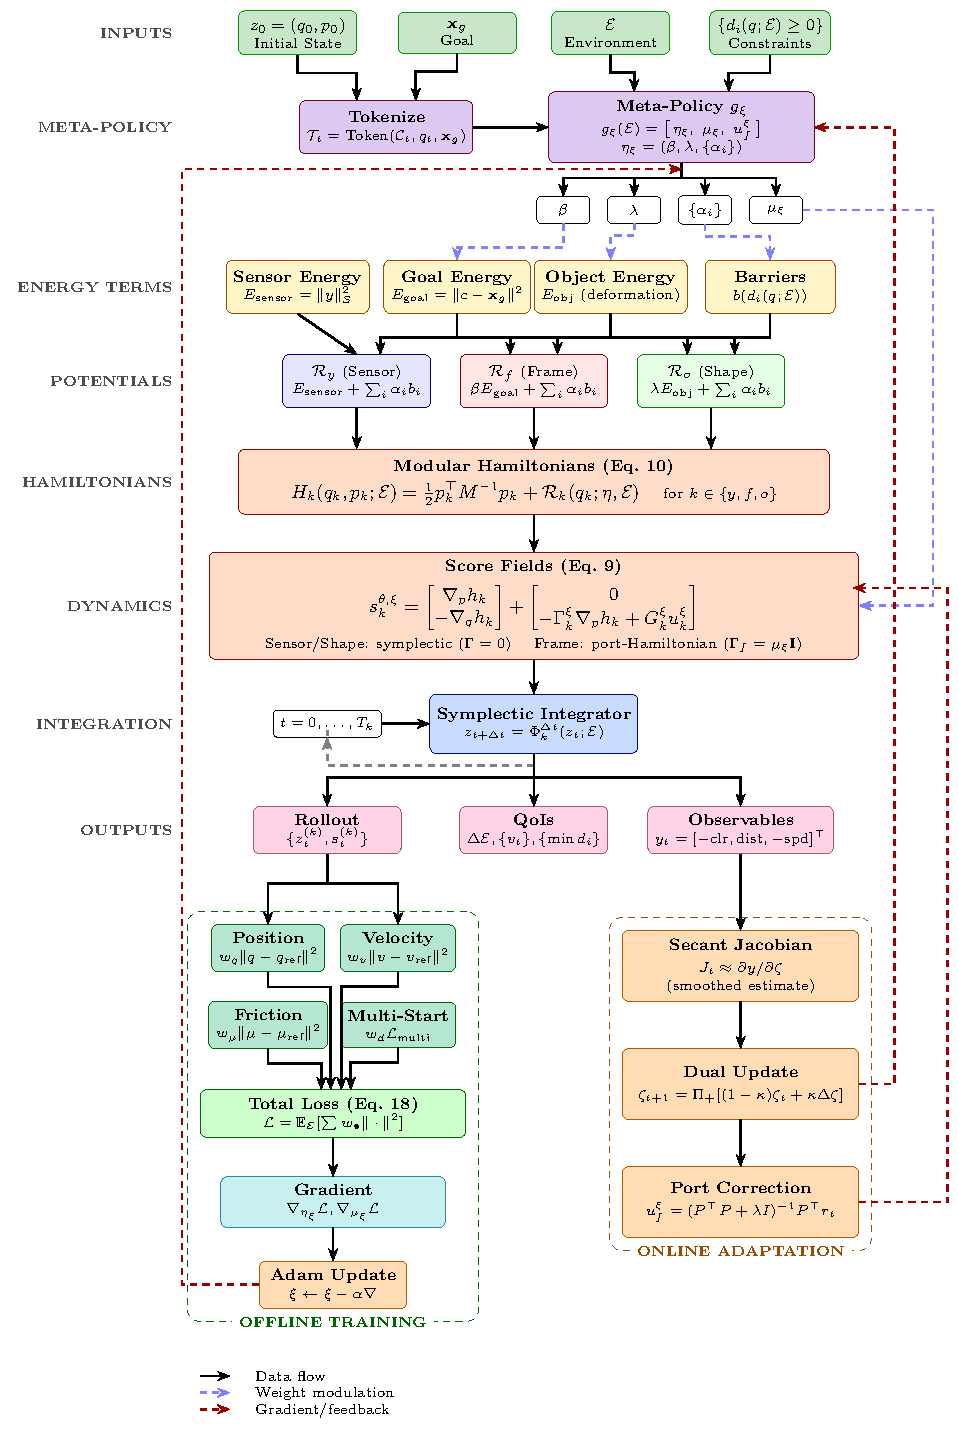
\includegraphics[width=0.72\linewidth]{flow.pdf}
\caption{\textbf{GRL--SNAM computational flow: sub-modular Hamiltonian structure with offline training and online adaptation.}
Given the current state \(z_0=(\vec{q}_0,p_0)\), goal \(\mathbf{x}_g\), and locally sensed environment context \(\mathcal{E}\) (obstacle constraints \(\{d_i(q;\mathcal{E})\ge 0\}\)), the navigator \(g_\xi\) tokenizes the active local information and outputs a small set of \emph{meta-parameters}: the nonnegative energy weights \(\eta_\xi=(\beta,\lambda,\{\alpha_i\})\), the frame dissipation \(\mu_\xi\), and an optional frame port input \(u_f^\xi\).
These parameters modulate a fixed library of interpretable energy terms (sensor cost, goal attraction, deformation, and barrier penalties) to form module-specific potentials \(\mathcal{R}_y,\mathcal{R}_f,\mathcal{R}_o\), which define the corresponding modular Hamiltonians
\(H_k(\vec{q}_k,p_k;\mathcal{E})=\tfrac12 p_k^\top M^{-1}p_k + \mathcal{R}_k(\vec{q}_k;\eta_\xi,\mathcal{E})\) (c.f.\ \cref{eq:module_template_hamiltonian}).
Each module induces a score (drift) field; sensor and shape follow conservative (symplectic) dynamics, while the frame module additionally includes dissipation and a nonconservative port term.
A symplectic integrator rolls out the dynamics for a short horizon, producing trajectories and quantities of interest (environment updates, velocities, and clearances) as well as low-dimensional observables \(y_t=[-\mathrm{clr}_t,\ \mathrm{dist}_t,\ -\mathrm{spd}_t]^\top\).
\emph{Offline training} (left branch) learns the mapping from context to meta-parameters by minimizing a supervised loss on position/velocity/friction, augmented with a multi-start robustness term near obstacles.
\emph{Online adaptation} (right branch) updates only the current meta-parameters using a smoothed secant Jacobian estimate to track the desired observables, and uses the residual to compute a corrective port input when energy reweighting alone is insufficient.
Arrows indicate (i) forward data flow, (ii) weight modulation from \(g_\xi\) into energies, and (iii) gradient/feedback pathways connecting rollouts to offline updates and online corrections.}
    \label{fig:full:loop:grl:snam}
\end{figure}


\paragraph{Learning $\eta_{\xi}(\mathcal{E}), \mu_\xi(\mathcal{E})$ through observation of Hamiltonian dynamics.}
Each submodule exposes a response map that provides integrated dynamics rollout and additional quantity of interests (QoI) as the feedback:
\[
\mathsf{R}_k:\ \big(H_k;\theta_k,\mathcal E, \xi)\ \longmapsto\ 
\{z_t^{(k)}, \mathrm{QoI}_k\}_{t=0}^{T_k},\qquad k\in\mathcal{K},
\]
where $T_k$ refers time scale for each submodule. To be more specific:
\begin{equation}
    \mathrm{QoI}_{y}=\Delta\mathcal{E}, \quad \mathrm{QoI}_{f}=\{v_t^{(f)}:=M_f^{-1}p_t^{(f)}\}_{t=0}^{T_f} ,\quad \mathrm{QoI}_{o}= \{\min_{i\in\mathcal{C}_t(\mathcal{E},q)} d_i(q_t^{(o)};\mathcal{E})\}_{t=0}^{T_o}.
\end{equation}

Namely, feedback QoIs are: environmental update, velocity observation, and min distance clearance (and thus collision violation). Additional QoIs, that can be deduced from $z_t^{(k)},s_t^{(k)}$, are not stated here explicitly. To train a policy that output $\eta_{\xi}(\mathcal{E})$ and $\mu_{\xi}(\mathcal{E})$ with different environments, we propose to minimize
\begin{equation}
\label{eq:meta_loss}
\begin{aligned}
\mathcal L(\eta_\xi,\mu_\xi)
= \mathbb{E}_{\mathcal{E}}\left[
w_{q}\big\|\vec{q}-\vec{q}_{ref}\big\|_2^2
\;+\;
w_{v}\big\|\vec{v}-\vec{v}_{ref}\big\|_2^2
\;+\;
w_{\mu}\big\|\mu-\mu_{ref}\big\|_2^2
\;+\;
w_{d}\ \mathcal L_{\text{multi}}\right].
\end{aligned}
\end{equation}
where $\mathcal L_{\text{multi}}$ is a short multi-start robustness penalty that re-rolls from perturbed $q_t^{(k)}$ seeds near obstacles to discourage brittle $\eta_{\xi}(\mathcal{E})$ and $\mu_{\xi}(\mathcal{E})$ (details are addressed in Algorithm \ref{alg:meta_training}), and $w_{\bullet}\!\ge\!0$ are user-input hyperparameters. The training via \cref{eq:meta_loss} can be conducted offline, component-wise, or even fine-tuned online, but we state that it is important to fully utilize the instantaneous response from a real navigation scenario which provides the scheme of per-scneario online correction even when $\eta_\xi(\mathcal{E})$ and $\mu_\xi(\mathcal{E})$ are properly trained under large-scale simulated dataset with reference potentials.

\begin{algorithm}[htbp]
\caption{Offline GRL-SNAM training of $\eta(\mathcal{E})$ and $\mu_{\xi}(\mathcal{E})$}
\label{alg:meta_training}
\begin{algorithmic}[1]
\Require dataset of different environments $\{\mathcal{E}, \alpha_{ref},\beta_{ref},\lambda_{ref},\mu_{ref}\}\in \mathcal D$, step range $T\!\in\!\{2,3,4,5,6\}$, short rollout trials $M$, time step $\Delta t$, weights $w_{\bullet}$
\State Initialize $\xi$
\For{epoch $=1,2,\dots$}
  \For{batch $\mathcal B\subset\mathcal D$}
    \State Sample $(q_0,p_0)$ per scene $\mathcal{E}$ in $\mathcal{B}$
    \State Build \textbf{tokens} from active constraints $\mathcal{C}_t(\mathcal{E},q_0)$, goal $\vec{x}_g$, and current $(q_0,p_0)$
     \State $(\{\alpha_j\},\beta)\gets \eta_\xi(\textbf{tokens}),\quad \mu\gets \mu_{\xi}(\textbf{tokens})$
     \For{$m=1,2,\dots,M$}
    \State Sample a near obstacle point $\tilde{q}_0$, initialize $\tilde{p}_0$ towards nearest obstacle at $\tilde{q}_0$.
    \State Integrate \cref{eq:module_score_field} for $T$ steps from $(\tilde{q}_0,\tilde{p}_0)$. \State \Comment{e.g. {Leapfrog}}
    \State Compute $clr\gets \min_{i,t} d_i(\tilde{q}_t;\mathcal{E})$
    \State Compute $\mathcal L_{\text{multi}}\gets\mathcal{L}_{\text{multi}}+\frac{1}{M}b\!\left(r_{min}-\mathrm{clr},\hat{d}\right).$ \State \Comment{$r_{min}$ refers minimal radius of robot object.}
    \EndFor
    \State Integrate \cref{eq:module_score_field} for $T_k$ steps from $(q_0,p_0)$
    \State Evaluate loss $\mathcal L(\eta_\xi,\mu_\xi)$ in \cref{eq:meta_loss}\State Update $\eta_\xi,\mu_\xi$ using  $\nabla_{\eta_\xi}\mathcal L$ and $\nabla_{\mu_\xi}\mathcal L$   \Comment{ Uncertainty hyperpaprameter weighted}
  \EndFor
\EndFor
\end{algorithmic}
\end{algorithm}


\begin{figure}[htbp]
  \centering
  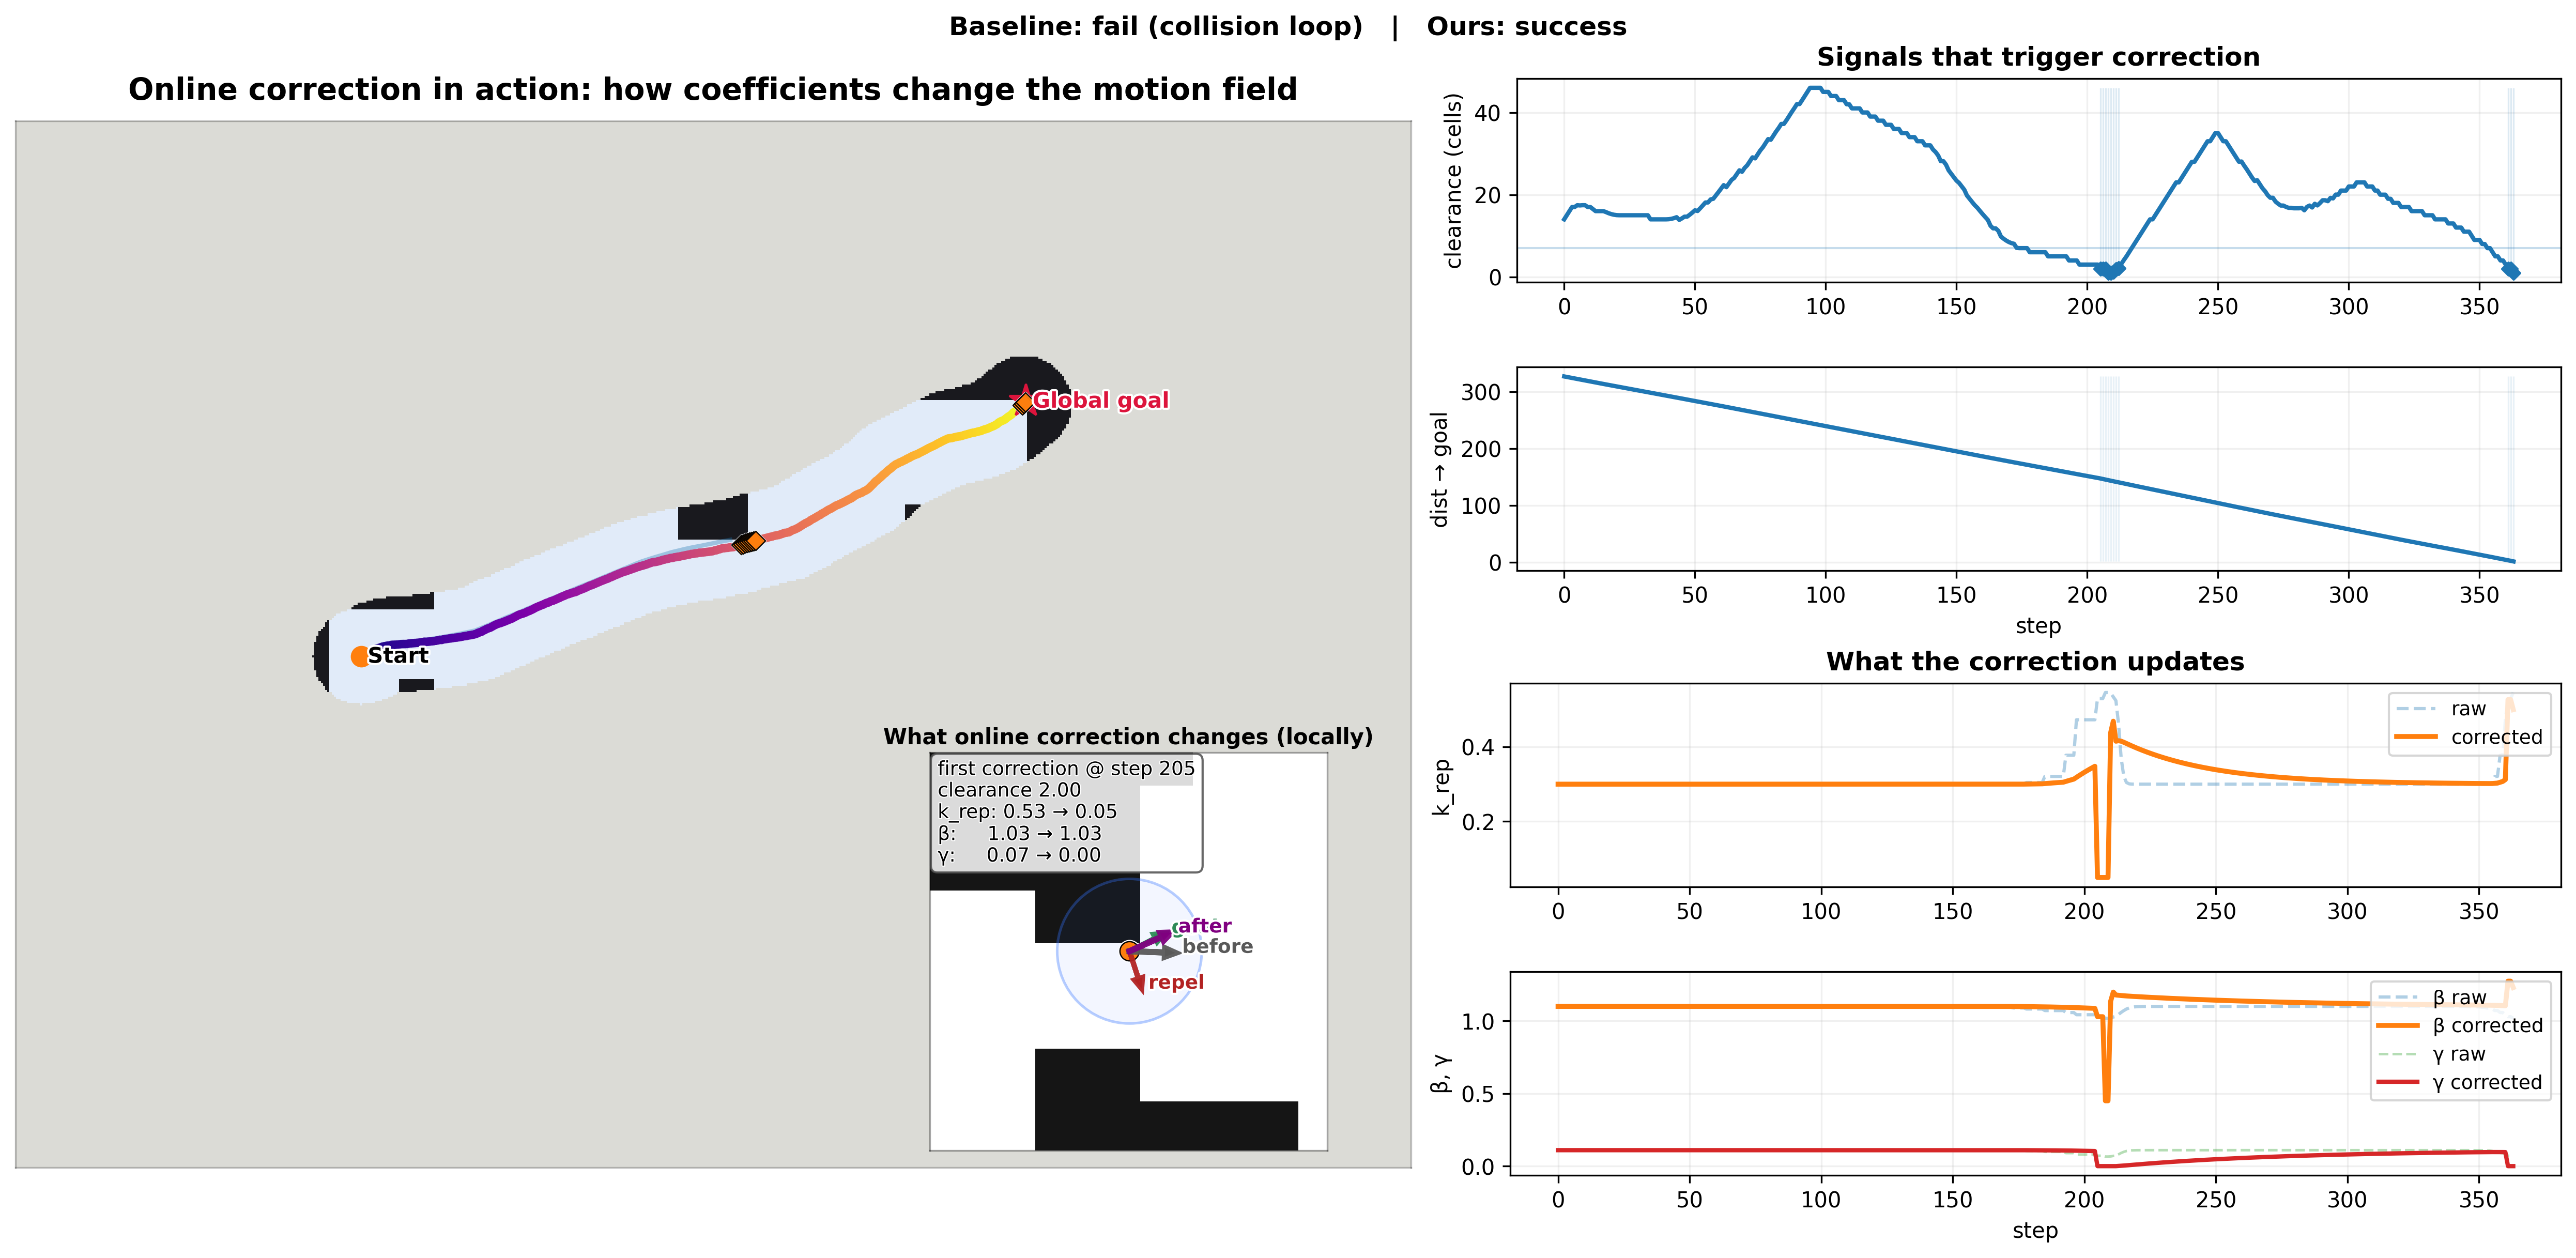
\includegraphics[width=\linewidth]{teaser_online_correction_mechanism.png}
\caption{\textbf{Online correction mechanism (Sec.~\ref{subsec:navigator_meta_learner}).}
{Left: a representative rollout where the frozen baseline enters a collision loop, while GRL--SNAM reaches the global goal by applying local corrections at detected failure points; the inset visualizes the first correction as a change in the local motion field (goal-seeking plus obstacle repulsion) around the active obstacles.
Right: the observable vector \(y_t=[-\mathrm{clr}_t,\ \mathrm{dist}_t,\ -\mathrm{speed}_t]^\top\) used for triggering/adaptation, with shaded bands marking correction events.
Bottom-right: the corresponding parameter updates i.e.; the dual weights \(\tilde{\eta}_t=[\beta_t,\ \lambda_t,\ \alpha_{t,\mathcal I_t}]^\top\) (active-set barrier weights) and dissipation/port terms \((\mu_t,\ u_{f,t}^\xi)\) show how the navigator performs lightweight, stage-local updates to the Hamiltonian-shaped policy to restore safety (clearance) while maintaining goal progress.}}
  \label{fig:online-correction-mechanism}
\end{figure}


\paragraph{Online Adaptation of $g_{\xi}(\mathcal{E})$ via QoIs}
We state how response map for each environment can yield a correction term under online navigation scenario. Given response $\mathsf{R}_k$ at time $t$ we construct an \emph{observable} measurement vector and its reference goal:
\[
y_t \;=\; \begin{bmatrix}
-\,\mathrm{clr}_t \\[2pt]
\mathrm{dist}_t \\[2pt]
-\,\mathrm{speed}_t
\end{bmatrix}\in\mathbb R^3,
\qquad
y_t^\star \;=\; \begin{bmatrix}
-\,m_{\mathrm{safe}}\\[2pt]
\mathrm{dist}_t-\varepsilon_{\mathrm{prog}}\\[2pt]
-\,\max\big(\mathrm{speed}_t,\ \mathbf 1_{\{\mathrm{clr}_t\ge m_{\mathrm{safe}}\}}\,v_{\min}\big)
\end{bmatrix},
\]
where $\mathrm{clr}$ is the minimum clearance to inflated obstacles, $\mathrm{dist}$ is goal distance (to the global goal point), and $\mathrm{speed}=\|v\|$.  
We update only the \emph{active} barrier weights by selecting an index set $\mathcal I_t$ that represents nearby obstacles. Define the parameter vector
\[
\tilde{\eta}_t\;=\;\begin{bmatrix}\beta_t\\ \lambda_t\\\alpha_{t,\mathcal I_t} \end{bmatrix}\in\mathbb R^{2+|\mathcal I_t|}_{\,+}, \quad \zeta_t=[\tilde{\eta}_t,\mu_t].
\]

We denote an estimator of Jabocian $J_t=\frac{\partial y}{\partial \zeta_t}$ as  
\[
\widetilde J_t\;=\;\frac{(y_t-y_{t-1})(\zeta_t-\zeta_{t-1})^\top}{\|\zeta_t-\zeta_{t-1}\|_2^2+\varepsilon},
\qquad
J_t\;=\;\rho\,J_{t-1}+(1-\rho)\,\widetilde J_t,
\]
with smoothing $\rho\in[0,1)$ and $\varepsilon>0$. Then, given the desired observable change $\Delta y^{\mathrm{des}}_t:=y_t^\star-y_t$, one can upate meta-policy parameter via a Tiknohov-regularized least square steps:
\[
\Delta\zeta_t \;=\; \arg\min_{\Delta\zeta}\ \big\|J_t\Delta\zeta-\Delta y^{\mathrm{des}}_t\big\|_2^2
\;+\;\lambda\|\Delta\zeta\|_2^2,
\quad\Rightarrow\quad
\Delta\zeta_t=(J_t^\top J_t+\lambda I)^{-1}J_t^\top\Delta y^{\mathrm{des}}_t.
\]
This yields updated $\beta_{t+1}$, $\gamma_{t+1}$, and $\alpha_{t+1,i}$ for $i\in\mathcal I_t$ (inactive weights keep their previous values).
\[
\zeta_{t+1}\;=\;\Pi_{\mathbb R_+}\big((1-\vec{\kappa})\,\zeta_t+ \vec{\kappa}\,\Delta\zeta_{t}\big),\quad \vec{\kappa}_i\in[0,1).
\]

Since the update is a result of least square step, there exists residual:
\[
r_t \;=\; \Delta y^{\mathrm{des}}_t - J_t\,\Delta\zeta_t.
\]
The online port correction term can amend the energy change by solving another least square problem given port–observable sensitivity $P_t\approx\partial y/\partial u_f$:
\[
u_{f,t}^{\xi}
\;=\;\arg\min_{u\in\mathcal U}\ \big\|P_t u - r_t\big\|_2^2+\lambda_u\|u\|_2^2
\;=\;(P_t^\top P_t+\lambda_u I)^{-1}P_t^\top r_t,
\]
followed by componentwise clipping to a feasible box $\mathcal U$.
A simple choice is to use $P_t=\operatorname{diag}(0,0,\kappa_v)$ so that the port primarily regulates speed while the energy weights steer clearance and goal progress. We comment that richer $P_t$ can be learned online by the same secant recipe as $J_t$.



\paragraph{Multi-Scale Temporal Coordination}
\label{subsec:temporal_coordination}

The policies operate at natural temporal hierarchies, creating stable multi-scale coordination, as shown in \cref{fig:temporal_scales}. This temporal separation enables a \textbf{nested quasi-static approximation}: the fastest dynamics (reconfiguration) equilibrate within each frame update, and frame dynamics settle before the slower sensor policy evolves.
This hierarchy prevents destabilizing interactions across timescales 
while preserving the necessary coupling for coherent, coordinated behavior.


\begin{figure}[ht]
\centering
\resizebox{0.75\textwidth}{!}{
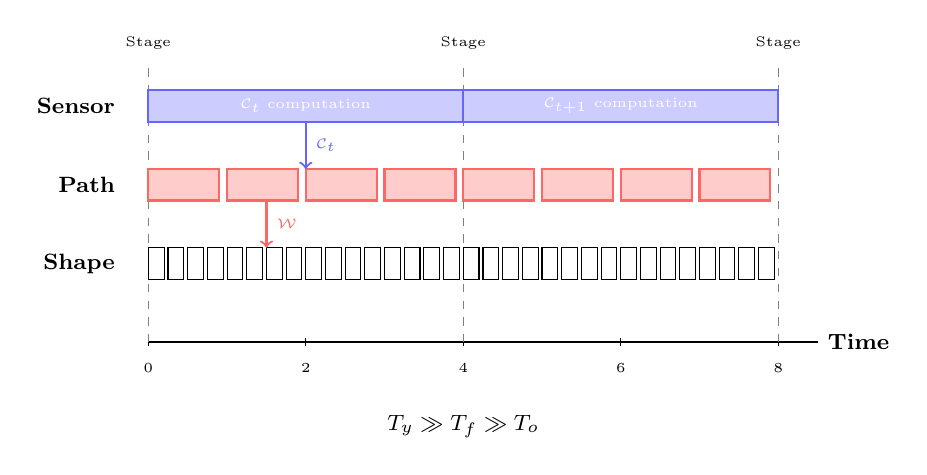
\begin{tikzpicture}[
  every node/.style={font=\footnotesize},
  sensor/.style={fill=blue!20, draw=blue!60, thick},
  path/.style={fill=red!20, draw=red!60, thick},
  shape/.style={fill=green!20, draw=green!60, thick},
  arrow/.style={->, thick, draw=gray!70},
]

% Compact timeline from 0 to 8
\draw[thick] (0,0) -- (8.5,0) node[right] {\textbf{Time}};
\foreach \x in {0,2,4,6,8} {
  \draw (\x,-0.05) -- (\x,0.05);
  \node[below] at (\x,-0.15) {\tiny $\x$};
}

% Stage boundaries
\foreach \x in {0,4,8} {
  \draw[dashed, gray] (\x,0) -- (\x,3.5);
  \node[above] at (\x,3.6) {\tiny Stage};
}

% Sensor (LOW frequency) - once per stage
\node[left] at (-0.3,3) {\textbf{Sensor}};
\draw[sensor] (0,2.8) rectangle (4,3.2);
\node[white] at (2,3) {\tiny $\mathcal{C}_t$ computation};
\draw[sensor] (4,2.8) rectangle (8,3.2);
\node[white] at (6,3) {\tiny $\mathcal{C}_{t+1}$ computation};

% Path (MEDIUM frequency) - multiple per stage  
\node[left] at (-0.3,2) {\textbf{Path}};
\foreach \x in {0,1,2,3} {
  \draw[path] (\x,1.8) rectangle (\x+0.9,2.2);
}
\foreach \x in {4,5,6,7} {
  \draw[path] (\x,1.8) rectangle (\x+0.9,2.2);
}

% Shape (HIGH frequency) - continuous adaptation
\node[left] at (-0.3,1) {\textbf{Shape}};
\foreach \x in {0,0.25,0.5,0.75,1,1.25,1.5,1.75,2,2.25,2.5,2.75,3,3.25,3.5,3.75} {
  \draw(\x,0.8) rectangle (\x+0.2,1.2);
}
\foreach \x in {4,4.25,4.5,4.75,5,5.25,5.5,5.75,6,6.25,6.5,6.75,7,7.25,7.5,7.75} {
  \draw(\x,0.8) rectangle (\x+0.2,1.2);
}

% Information flow arrows
\draw[arrow, blue!60] (2,2.8) -- (2,2.2) node[midway,right] {\tiny $\mathcal{C}_t$};
\draw[arrow, red!60] (1.5,1.8) -- (1.5,1.2) node[midway,right] {\tiny $\mathcal{W}$};


\node[below] at (4,-0.8) {$T_{y} \gg T_{f} \gg T_{o}$};
\end{tikzpicture}
}
\caption{Temporal hierarchy. Sensor policy operates at low frequency (once per stage), establishing environmental constraints $\mathcal{C}_t$. Path policy operates at medium frequency within each stage, computing waypoints $\mathcal{W}$. Shape policy operates at high frequency, continuously adapting at each integration step. This creates a natural hierarchy where slow sensor updates provide stable constraints for faster path and shape adaptations.}
\label{fig:temporal_scales}
\end{figure}

\section{Hyperelastic Ring Robot Model}
\label{app:hyperelastic_model}

Our framework in Sec.~\ref{sec:method} is agnostic to the underlying robot body: the score-based policies $\{\pi_y,\pi_f,\pi_o\}$ only assume access to a local context $\mathcal{C}_t$ , a reduced state $z_t$ and a modular hamiltonian proposal. For experiments, we instantiate this framework on a planar \emph{hyperelastic ring} that must squeeze through clutter and narrow passages. In this domain, the shape policy $\pi_o$ acts on a low-dimensional shape state
\[
z_o(t) = \big(s(t), p_s(t)\big),
\]
where $s(t)\!>\!0$ is a uniform scale, and one denote $\mathbf{o}(t)\in\mathbb{R}^2$ as the ring center coincide with robot frame center $\vec{c}$.

\paragraph{Design rationale.}
We choose a hyperelastic ring with a spline boundary for three reasons that match the Hamiltonian formulation in Sec.~\ref{sec:method}:
(i) it is the simplest soft body that \emph{provably requires} shape change to solve our benchmarks (a rigid disc of any fixed radius cannot pass through the same bottlenecks), so deformation and collision–clearance trade-offs cannot be “faked” by rigid planning alone;
(ii) the reduced state $s$ provides a low-dimensional, analytically tractable testbed for the energy decomposition in \cref{eq:module_template_hamiltonian}, letting us study Hamiltonian energy shaping and meta-weights $(\beta,\lambda,\{\alpha_i\})$ without confounding internal DOF; and

Thus, the hyperring model is not a restriction of GRL--SNAM, but a controlled, low-DOF instantiation that stresses exactly the squeezing and clearance behaviors we target.

\begin{figure}[htbp]
\centering
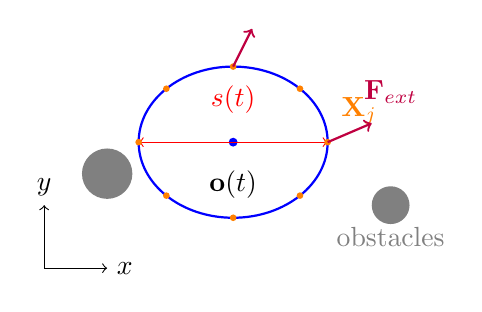
\begin{tikzpicture}[scale=0.8]
% Robot ring
\draw[thick,blue] (0,0) ellipse (1.5 and 1.2);
\fill[blue] (0,0) circle (2pt);
\node[below] at (0,-0.3) {$\mathbf{o}(t)$};
% Scale arrows
\draw[<->,red] (-1.5,0) -- (1.5,0);
\node[above,red] at (0,0.3) {$s(t)$};

\foreach \angle in {0,45,90,135,180,225,270,315} {
  \fill[orange] ({1.5*cos(\angle)},{1.2*sin(\angle)}) circle (1.5pt);
}
\node[orange] at (2,0.5) {$\mathbf{X}_j$};
% Force vectors
\draw[->,purple,thick] (1.5,0) -- (2.2,0.3);
\draw[->,purple,thick] (0,1.2) -- (0.3,1.8);
\node[purple] at (2.5,0.8) {$\mathbf{F}_{\text{ext}}$};
% Obstacles
\fill[gray] (2.5,-1) circle (0.3);
\fill[gray] (-2,-0.5) circle (0.4);
\node[gray] at (2.5,-1.5) {obstacles};
% Coordinate system
\draw[->] (-3,-2) -- (-2,-2) node[right] {$x$};
\draw[->] (-3,-2) -- (-3,-1) node[above] {$y$};
\end{tikzpicture}
\caption{Hyperelastic ring instantiation of the generic shape policy $\pi_o$.
The reduced configuration $s$ is mapped to spline samples $\mathbf{X}_j$ where policy-induced forces act.}
\label{fig:hyperelastic_ring}
\end{figure}

\paragraph{Geometric Representation of Hyperelastic Ring}

We represent the boundary of the hyperelastic ring object by a periodic cubic B-spline with $n_{\text{ctrl}}$ control points
\begin{equation}
\mathbf{S}(u) = \sum_{i=1}^{n_{\text{ctrl}}} N_{i,3}(u)\,\mathbf{P}_i,
\quad u \in [0,1],
\end{equation}
where $N_{i,3}$ are $C^2$-continuous B-spline basis functions.
This choice provides a smooth closed curve with well-defined normals and curvature, and allows fast evaluation through precomputed matrices. A reference unit ring is initialized as
\begin{equation}
\mathbf{P}_{0,i} 
= r_{\text{base}}
\begin{bmatrix}
\cos(2\pi i/n_{\text{ctrl}}) \\
\sin(2\pi i/n_{\text{ctrl}})
\end{bmatrix},
\end{equation}
and transformed to world coordinates by a similarity transform
\(\mathbf{P}_i(t) = \mathbf{o}(t) + s(t)\,\mathbf{P}_{0,i}.\)
For numerical evaluation we precompute spline matrices $B,D\in\mathbb{R}^{K\times n_{\text{ctrl}}}$ and sample $K$ points on the boundary
\begin{equation}
\mathbf{X}_j(t) = \sum_{i} B_{ji}\,\mathbf{P}_i(t), 
\quad
\mathbf{X}'_j(t) = \sum_{i} D_{ji}\,\mathbf{P}_i(t),
\end{equation}
with arc lengths $\ell_j = \|\mathbf{X}'_j\|$ and unit tangents $\hat{\mathbf{T}}_j = \mathbf{X}'_j / \ell_j$.
We use uniform quadrature weights $\omega_j= 1/K$.


\paragraph{{Shape Sub-Modular Hamiltonian.}}

In this domain, the generic Hamiltonian from \cref{eq:module_template_hamiltonian} specializes to
\begin{equation}
\mathcal{H}_{\text{o}}(z_o;\mathcal{E}_\tau)
=\frac{1}{2}M_s^{-1} p_s^2 
+ \mathcal{R}_o(q_o;\mathcal{E}_t),
\end{equation}
where $M_s$ refers a fixed ``mass" term of scale and $p_s=M_s^{-1}\dot{s}$ refers conjugate momenta.
We match the navigation specialization in \cref{eq:module_template_potential:o} by defining the barrier potentials $b(d_i(q,\mathcal{E}))$ and object intrinsic energy $E_{\mathrm{obj}}$ for deformation.

\paragraph{{Barrier potentials.}}
The sensor policy $\pi_y$ exposes { weighted point obstacles} $(\mathbf{c}_i,r_i,w_i)$ in $\mathcal{C}_t$ from $\mathcal{E}$. Here $\vec{c}_i$ denotes the center of objects and $r_i$ denotes the distance. $w_i$ denotes the scale of obstacles. For each sample point $\mathbf{X}_j$ we compute distances \(d_{ji} = \|\mathbf{X}_j - \mathbf{c}_i\| - r_i,\)
and accumulate an Incremental Potential Contact (IPC, \citet{li2020incremental}) barrier function:
\begin{equation}
d_i(q,\mathcal{E}):=
\sum_{j=1}^K \omega_j \ell_j  w_k b_{\text{IPC}}(d_{jk};\hat{d}),
\end{equation}
with $b_{\text{IPC}}(\cdot)$ in the standard piecewise form
\begin{equation}
b_{\text{IPC}}(d;\hat{d}) =
\begin{cases}
-(d-\hat{d})^2(\log d - \log \hat{d}) & 0 < d < \hat{d},\\[2pt]
0 & d \geq \hat{d},\\[2pt]
V_{\text{penalty}} & d \leq 0.
\end{cases}
\end{equation}
 
The term $\hat{d}$ refers the contact distance thresholding while $V_{\text{penalty}}$ is a user-specified constant that penalize penetration. This is a concrete instantiation of the barrier term in \cref{eq:barrier_shaped_cost}, with IPC chosen because its differential yields near obstacle contact forces and time integrations resembles physical-world behaviors of an elastic object. { We provide \cref{cor:ipc_from_logbarrier} to justify IPC potentials are also a valid barrier function that maintains the conclusions addressed in \cref{prop:barrier_convergence}.}
\paragraph{Object potential.}

Let $A_{\text{ref}}$ denote the reference rest area of the ring. We denote the scaled area $A(s)= s^2 A_{\text{ref}}$.
We compute the minimal clearance \(d_{\min}:=\min_{j,i}~\{d_{ji}\},\)
and use it to define a clearance-dependent scale target 
\begin{equation}
s_{\text{target}}
:=
s_0 + (1-s_0)\tanh\big(\delta\,\max(d_{\min},0)\big),
\label{eq:def:radius:target}
\end{equation}
which encourages compression in tight passages while keeping the ring expanded in free space:
for large $d_{\min}$, $s_{\text{target}}$ shall be close to $1$, while for lower clearance the target shrinks smoothly.
The bulk potential is thus defined as
\begin{equation}
{E}_{\text{obj}}(q):=\mathcal{U}_{bulk}(s;d_{\min})
=
\frac{k_{\text{bulk}}}{2}\big(A(s) - A(s_{\text{target}})\big)^2.
\end{equation}
This realizes $E_{\mathrm{obj}}$ with a \emph{single} deformation DOF (scale $s$), striking a balance between expressivity (squeezing is possible) and the low-dimensional Hamiltonian search space assumed in Sec.~\ref{subsec:problem_formulation}. The three policies $\{\pi_y,\pi_f,\pi_o\}$ interact with the ring exactly at the level of boundary samples, in a way that mirrors the abstract modular decomposition of $\mathcal{R}$.

